\documentclass[a4paper,11pt]{article}

% Kodovani (cestiny) v dokumentu: utf-8
%\usepackage[cp1250]{inputenc}	% Omezena stredoevropska kodova stranka, pouze MSW.
\usepackage[utf8]{inputenc}	% Doporucujeme pouzivat UTF-8 (unicode).

\usepackage[margin=2cm]{geometry}
\newtoks\jmenopraktika \newtoks\jmeno \newtoks\datum
\newtoks\obor \newtoks\skupina \newtoks\rocnik \newtoks\semestr
\newtoks\cisloulohy \newtoks\jmenoulohy
\newtoks\tlak \newtoks\teplota \newtoks\vlhkost

\jmenopraktika={Fyzikální praktikum 3}
\jmeno={Lukáš Lejdar}
\datum={20. května 2025}
\obor={F}
\skupina={Út 14:00}

\cisloulohy={6}
\jmenoulohy={Zeemanův jev}

\tlak={101{,}35}
\teplota={21,1}
\vlhkost={47,7}


%%%%%%%%%%% Uzitecne balicky:
\usepackage[czech]{babel}

\usepackage{graphicx}
\usepackage{amsmath}
\usepackage{xspace}
\usepackage{url}
\usepackage{indentfirst}
\usepackage{wrapfig}
\usepackage{xcolor}
\usepackage{subfig}
\usepackage{subcaption}
\usepackage{enumitem}
\usepackage{tikzsymbols}
\usepackage{newfloat}

\DeclareFloatingEnvironment[fileext=lof]{graph}
\captionsetup[graph]{labelformat=simple, labelsep=colon, name=Graf}

%%%%%% Zamezeni parchantu:
\widowpenalty 10000 \clubpenalty 10000 \displaywidowpenalty 10000
%%%%%% Parametry pro moznost vsazeni vetsiho poctu obrazku na stranku
\setcounter{topnumber}{3}	  % max. pocet floatu nahore (specifikace t)
\setcounter{bottomnumber}{3}	  % max. pocet floatu dole (specifikace b)
\setcounter{totalnumber}{6}	  % max. pocet floatu na strance celkem
\renewcommand\topfraction{0.9}	  % max podil stranky pro floaty nahore
\renewcommand\bottomfraction{0.9} % max podil stranky pro floaty dole
\renewcommand\textfraction{0.1}	  % min podil stranky, ktery musi obsahovat text
\intextsep=8mm \textfloatsep=8mm  %\intextsep pro ulozeni [h] floatu a \textfloatsep pro [b] or [t]

% Tecky za cisly sekci:
\renewcommand{\thesection}{\arabic{section}.}
\renewcommand{\thesubsection}{\thesection\arabic{subsection}.}
% Jednopismenna mezera mezi cislem a nazvem kapitoly:
\makeatletter \def\@seccntformat#1{\csname the#1\endcsname\hspace{1ex}} \makeatother
%
\newcommand{\vsn}[4]{\ensuremath{#1 =} #2(#3)\,#4}
\newcommand{\vrn}[6]{\ensuremath{#1 =} (#2 $\pm$ #3)\,#4 ($p=$ #5\,\%, $\nu=$ #6)}

\newcommand*\circled[1]{\tikz[baseline=(char.base)]{
		\node[shape=circle,draw,inner sep=1pt] (char) {#1};}}

%%%%%%%%%%%%%%%%%%%%%%%%%%%%%%%%%%%%%%%%%%%%%%%%%%%%%%%%%%%%%%%%%%%%%%%%%%%%%%%
% Zacatek dokumentu
%%%%%%%%%%%%%%%%%%%%%%%%%%%%%%%%%%%%%%%%%%%%%%%%%%%%%%%%%%%%%%%%%%%%%%%%%%%%%%%

\begin{document}

\thispagestyle{empty}

{
\begin{center}
\sf 
{\Large Ústav fyziky a technologií plazmatu Přírodovědecké fakulty Masarykovy univerzity} \\
\bigskip
{\huge \bfseries FYZIKÁLNÍ PRAKTIKUM} \\
\bigskip
{\Large \the\jmenopraktika}
\end{center}

\bigskip

\sf
\noindent
\setlength{\arrayrulewidth}{1pt}
\begin{tabular*}{\textwidth}{@{\extracolsep{\fill}} l l}
\large {\bfseries Zpracoval:}  \the\jmeno & \large  {\bfseries Naměřeno:} \the\datum\\[2mm]
\large  {\bfseries Obor:} \the\obor  \hspace{40mm}  {\bfseries Skupina:} \the\skupina %
&\large {\bfseries Testováno:}\\
\\
\hline
\end{tabular*}
}

\bigskip

{
\sf
\noindent \begin{tabular}{p{4cm} p{0.6\textwidth}}
\Large  Úloha č. {\bfseries \the\cisloulohy:} \par
\smallskip
&\Large \bfseries \the\jmenoulohy  \\[2mm]
\end{tabular}
}

\vskip1cm

\section{Úvod}

Cílem úlohy je změřit rozdíl vlnových délek při štěpení spektrálních čar kadmiové lampy v přítomnosti magnetického pole pomocí Fabr-Perotova interferometru. Z naměřených dat dopočítáme Bohrův magneton $ \mu_B $ a zjistíme jakou polarizaci má takto vyzářené světlo. 

 
\section{Teorie}

\subsection{Fabry-Perotův interferometr}

Fabry-Perotův interferometr je obvykle několik mm tlustá průhledná destička pokrytá na obou stranách vrstvou odrážející většinu dopadajícího záření. Při průchodu paprsku interferometrem potom dochází k násobným odrazům a následné interferenci série propuštěného záření podobně jako je to schematicky znázorněné na Obrázku 1.

\begin{table}[htpb]
    \captionsetup{type=figure}
    \begin{minipage}{.45\linewidth}
        \centering
        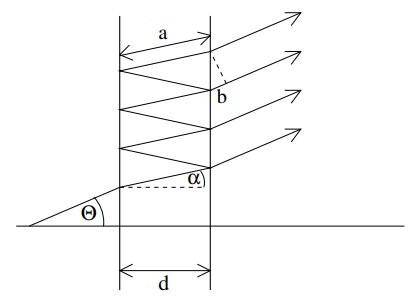
\includegraphics[width=0.8\textwidth]{fabry_schema.jpg}
        \caption{Chod paprsků ve Fabry-perotově interferometru. }
    \end{minipage} 
    \hfill
    \begin{minipage}{.45\linewidth}
        \centering
        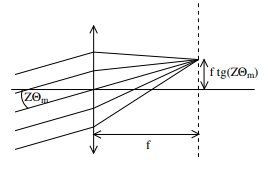
\includegraphics[width=0.8\textwidth]{zorbrazeni_schema.jpg}
        \caption{Zobrazení interferenčního obrazce spojkou. }
    \end{minipage} 
\end{table}

Rozdíl optických drah dvou sousedních vycházejících paprsků má velikost $ 2 n d \cos \alpha_m $, takže podmínka konstruktivní interference v aproximaci pro malé úhly je 

\begin{equation}
m \lambda = 2 n d \cos \alpha_m \approx 2 n d \left( 1 - \frac{\alpha^2_m}{2} \right)
\end{equation}

\noindent
kde $ d $ je šířka interferometru, $ m $ je některé celé číslo a $ \lambda $ vlnová délka světla. Ke konstruktivní interferenci tedy dochází jen pro některé úhly dopadu $ \Theta_m \approx n \alpha_m $, takže světlo dopadající na interferometr musí částečně divergovat.  Paprsek dál prochází skrz dvě spojky fungující jako dalekohled o zvětšení $ Z $ a nakonec do objektivu kamery o ohniskové vzdálenosti $ f $. Velikost obrazu $ r_m $ je potom

\begin{equation}
r_m = f \tan ( Z \Theta_m ) \approx f Z \Theta_m \approx f Z n \alpha_m
\end{equation}

\noindent
a dosazením z (1) dostáváme vztah

\begin{equation}
    r_m = f Z n \sqrt{ 2 - \frac{m\lambda}{nd}  }.
\end{equation}

Pokud na interferometr dopadá světlo o dvou velmi blízkých vlnových délkách $ \lambda_a $ a $ \lambda_b $, bude se rozdíl čtverců jejich poloměrů obrazu řádu $ m $ lišit o 

\begin{equation}
r^2_{b,m} - r^2_{a,m} = (f Z n)^2 \frac{m}{ n d} \left( \lambda_a - \lambda_b    \right).
\end{equation}

\noindent
A podělením výrazem

\begin{align*}
    r^2_{a,m}  - r^2_{a,m+1} = (fZn)^2 \frac{\lambda_a}{nd} 
\end{align*}

\noindent
dostáváme vztah pro rozdíl vlnočtů 

\begin{align*}
    \frac{ r^2_{b,m} - r^2_{a,m} }{ r^2_{a,m}  - r^2_{a,m+1} } &= \frac{m}{ \lambda_a} \left( \lambda_a - \lambda_b    \right) \\
    \frac{ r^2_{b,m} - r^2_{a,m} }{ r^2_{a,m}  - r^2_{a,m+1} } &= m \lambda_b \left( \frac{1}{\lambda_b} - \frac{1}{\lambda_a}     \right) \\
    \frac{ r^2_{b,m} - r^2_{a,m} }{ r^2_{a,m}  - r^2_{a,m+1} } & \approx 2 n d  \left( \frac{1}{\lambda_b} - \frac{1}{\lambda_a}     \right) \\
\end{align*}

\noindent
Rozdíl energie dvou paprsků o různých vlnových délkách je potom

\begin{equation}
\Delta E = \frac{hc}{2nd} \frac{ r^2_{b,m} - r^2_{a,m} }{ r^2_{a,m}  - r^2_{a,m+1} } 
\end{equation}

\subsection{Normální Zeemanův jev}

Každý i-tý elektron v obalu atomu má svůj magnetický moment $ \vec{\mu}_{ji} $ daný jeho kvantovými čísly, nebo se nachází v superpozici více možných stavů. Přivedením magnetického pole $ B \hat{z} $ na atom dojde ke kolapsu superpozice celkového magnetického momentu $ \vec{\mu}_J = \sum_i  \vec{\mu}_{ji} $ a je možné sledovat štěpení spektrálních čar, kvůli nepatrným rozdílům potenciální energie $ U $ jednotlivých stavů s různými momenty $ \vec{\mu}_J $.

\begin{equation}
U = - \vec{\mu}_J B \hat{z}
\end{equation}

V případě Normálního Zeemanova jevu nastává přechod mezi singletovými stavy, kde celkový spin elektronů je nulový a proto je celkový moment hybnosti daný pouze orbitálním momentem.

\begin{equation}
    \vec{J} = \vec{L} \quad \quad | \vec{L} | = \sqrt{L(L + 1)}  \hbar \quad \quad L_z = m_l \hbar
\end{equation}

\noindent
Magnetický moment potom spočítáme podle vztahu

\begin{equation}
\vec{\mu}_J = - g_J \frac{e}{2 m_e} \vec{J}
\end{equation}

\noindent
kde $ m_e $ a $ e $ je hmotnost a náboj elektronu a $ g_J $ je Landého faktor, který pro $ S=1 $ a $ L=J $ vychází $ g_J = 1 $. Dosazením do vztahu (6) dostáváme

\begin{equation}
U = - m_l \frac{e \hbar}{2m_e} B = - m_l \mu_B B
\end{equation}

\noindent

kde $ \mu_B $ je Bohrův magneton. V praktiku budeme pozorovat spektrum kadmia, které má v základním stavu plný poslední valenční orbital $ 4d^{10} $ a proto má i nulový celkový spin, který se při přechodech nemění. V jeho spektru můžeme nalézt čáru s vlnovou délkou $ \lambda = 643 $ nm, která odpovídá přechodu mezi orbitaly $ 4d^{10}5s5d \rightarrow 4d^{10}5s5p   $, při kterém platí výběrové pravidlo $ \Delta m_l = 0, \pm 1 $ a dochází ke štěpení energie stavů 

\begin{equation}
\text{pro } \Delta m = \pm 1 \quad  \quad  \Delta E = \pm \mu_B B
\end{equation}

Prostřední čára vyzářená při $ \Delta m = 0 $  se označuje $ \pi $ a takové fotony nutně musí mít složku momentu hybnosti $ j_z = 0 $, takže se muže šířit jen ve směru kolmém na $ \hat{z} $ a bude lineárně polarizované ve směru $ \hat{z} $. Čáry odpovídající $ \Delta m = \pm 1 $ se označují $ \sigma^\pm $ a budou kruhově polarizované v ploše $ xy $ s  $ j_z = \pm \hbar $. Pokud je pozorujeme ve směru kolmém k $ \hat{z} $, potom se plocha $ xy $ projektuje na přímku a světlo je lineárně polarizované kolmo na osu $ \hat{z} $. 

\subsection{Anomální Zeemanův jev}

Anomální Zeemanův nastává při přechodu mezi stavy s nenulovým spinem. V takovém případě se změna magnetického momentu rozkládá na Orbitální i spinovou složku a štěpení probíhá mnohonásobně štěpení spektrální čáry.

\section{Postup měření}

Kadmiová lampa s dvěma elektromagnety je umístěná na otočném stolku ve kterém jsou otvory kterými je možné vyzářené světlo pozorovat buď kolmo, nebo rovnoběžně s magnetickým polem. Na optické lavici je za stolkem postupně umístěna irisová clona , Fabry-Perotův interferometr a dalekohled složený ze dvou spojek o ohniskových vzdálenostech $ f_1 = 30 $ cm a $ f_2 = 5  $ cm, které obraz zvětšují $ Z = 30  / 5 = 6 $ krát a za nimi ještě filtr červeného světla s kamerou. Poloměry interferenčních kroužků se odečítají digitálně z fotek a ke zjištění polarity světla můžu použít polarizátory, a čtvrtvlnnou nebo půlvlnnou destičku. 

\begin{figure}[htpb]
    \centering
    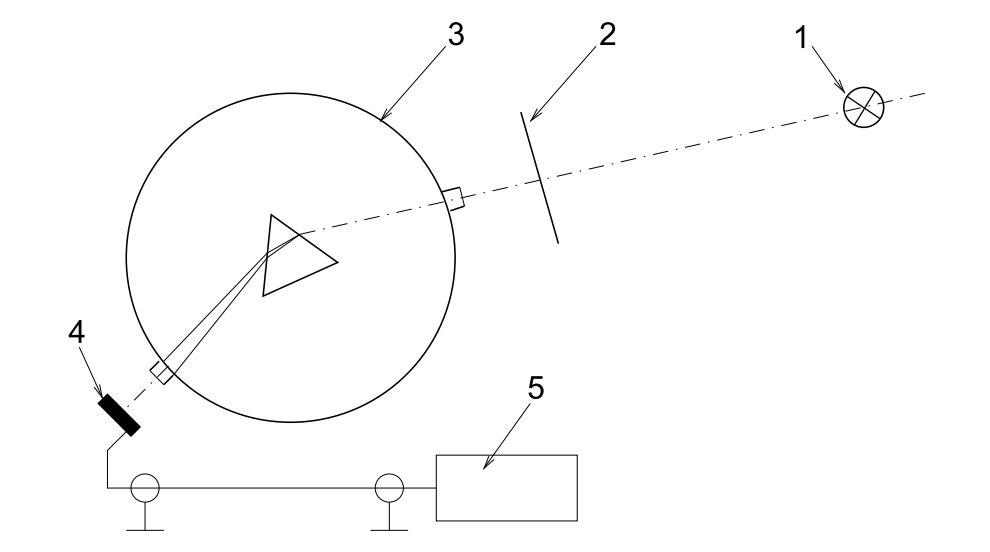
\includegraphics[width=0.9\textwidth]{aparatura.jpg}
    \caption{Schéma aparatury}
\end{figure}

\newpage

\section{Výsledky měření}

\subsection{Interpolace magnetické indukce}

Závislost intenzity magnetické indukce na proudu procházejícím cívkami uvnitř kadmiové lampy jsem dostal naměřenou v zadání skrz tabulku 1. Data jsem vykreslil do Grafu 1 a fitoval je polynomem třetího řádu $ B(I) = aI^3 + bI^2 + cI + d $ ze kterého vyšly parametry

\begin{align*}
    a &= 0.21 \pm 0.02 \text{ mTA}^{-3} &  c &= 5.0 \pm 2 \text{ mTA}^{-1} \\
    b &= 2.9 \pm 0.4 \text{ mTA}^{-2}  &     d &= 1.9 \pm 3 \text{ mT}
\end{align*}

\vspace{-20pt}

\begin{table}[htpb]
    \begin{minipage}{.45\linewidth}
    \centering
    \begin{tabular}{|c c|c c|}
        \hline
        $I$ (A) & $B$ (mT) & $I$ (A) & $B$ (mT) \\
        \hline
        1.03 & 73 & 4.66 & 295 \\
        1.89 & 124 & 5.05 & 319 \\
        2.60 & 166 & 5.53 & 348 \\
        2.97 & 188 & 6.06 & 381 \\
        3.86 & 248 & 6.54 & 409 \\
        7.10 & 444 & 8.06 & 500 \\
        7.50 & 468 & 8.47 & 524 \\
        8.96 & 549 & 9.50 & 573 \\
        9.95 & 594 & 10.46 & 613 \\
        \hline
    \end{tabular}
    \caption{Intenzita magnetického pole v závislosti na proudu. }
    \end{minipage} 
    \hfill
    \begin{minipage}{.5\linewidth}
        \centering
        \resizebox{\textwidth}{!}{ % GNUPLOT: LaTeX picture with Postscript
\begingroup
  \makeatletter
  \providecommand\color[2][]{%
    \GenericError{(gnuplot) \space\space\space\@spaces}{%
      Package color not loaded in conjunction with
      terminal option `colourtext'%
    }{See the gnuplot documentation for explanation.%
    }{Either use 'blacktext' in gnuplot or load the package
      color.sty in LaTeX.}%
    \renewcommand\color[2][]{}%
  }%
  \providecommand\includegraphics[2][]{%
    \GenericError{(gnuplot) \space\space\space\@spaces}{%
      Package graphicx or graphics not loaded%
    }{See the gnuplot documentation for explanation.%
    }{The gnuplot epslatex terminal needs graphicx.sty or graphics.sty.}%
    \renewcommand\includegraphics[2][]{}%
  }%
  \providecommand\rotatebox[2]{#2}%
  \@ifundefined{ifGPcolor}{%
    \newif\ifGPcolor
    \GPcolorfalse
  }{}%
  \@ifundefined{ifGPblacktext}{%
    \newif\ifGPblacktext
    \GPblacktexttrue
  }{}%
  % define a \g@addto@macro without @ in the name:
  \let\gplgaddtomacro\g@addto@macro
  % define empty templates for all commands taking text:
  \gdef\gplbacktext{}%
  \gdef\gplfronttext{}%
  \makeatother
  \ifGPblacktext
    % no textcolor at all
    \def\colorrgb#1{}%
    \def\colorgray#1{}%
  \else
    % gray or color?
    \ifGPcolor
      \def\colorrgb#1{\color[rgb]{#1}}%
      \def\colorgray#1{\color[gray]{#1}}%
      \expandafter\def\csname LTw\endcsname{\color{white}}%
      \expandafter\def\csname LTb\endcsname{\color{black}}%
      \expandafter\def\csname LTa\endcsname{\color{black}}%
      \expandafter\def\csname LT0\endcsname{\color[rgb]{1,0,0}}%
      \expandafter\def\csname LT1\endcsname{\color[rgb]{0,1,0}}%
      \expandafter\def\csname LT2\endcsname{\color[rgb]{0,0,1}}%
      \expandafter\def\csname LT3\endcsname{\color[rgb]{1,0,1}}%
      \expandafter\def\csname LT4\endcsname{\color[rgb]{0,1,1}}%
      \expandafter\def\csname LT5\endcsname{\color[rgb]{1,1,0}}%
      \expandafter\def\csname LT6\endcsname{\color[rgb]{0,0,0}}%
      \expandafter\def\csname LT7\endcsname{\color[rgb]{1,0.3,0}}%
      \expandafter\def\csname LT8\endcsname{\color[rgb]{0.5,0.5,0.5}}%
    \else
      % gray
      \def\colorrgb#1{\color{black}}%
      \def\colorgray#1{\color[gray]{#1}}%
      \expandafter\def\csname LTw\endcsname{\color{white}}%
      \expandafter\def\csname LTb\endcsname{\color{black}}%
      \expandafter\def\csname LTa\endcsname{\color{black}}%
      \expandafter\def\csname LT0\endcsname{\color{black}}%
      \expandafter\def\csname LT1\endcsname{\color{black}}%
      \expandafter\def\csname LT2\endcsname{\color{black}}%
      \expandafter\def\csname LT3\endcsname{\color{black}}%
      \expandafter\def\csname LT4\endcsname{\color{black}}%
      \expandafter\def\csname LT5\endcsname{\color{black}}%
      \expandafter\def\csname LT6\endcsname{\color{black}}%
      \expandafter\def\csname LT7\endcsname{\color{black}}%
      \expandafter\def\csname LT8\endcsname{\color{black}}%
    \fi
  \fi
    \setlength{\unitlength}{0.0500bp}%
    \ifx\gptboxheight\undefined%
      \newlength{\gptboxheight}%
      \newlength{\gptboxwidth}%
      \newsavebox{\gptboxtext}%
    \fi%
    \setlength{\fboxrule}{0.5pt}%
    \setlength{\fboxsep}{1pt}%
    \definecolor{tbcol}{rgb}{1,1,1}%
\begin{picture}(5040.00,3168.00)%
    \gplgaddtomacro\gplbacktext{%
      \csname LTb\endcsname%%
      \put(814,704){\makebox(0,0)[r]{\strut{}$0$}}%
      \put(814,1024){\makebox(0,0)[r]{\strut{}$0.1$}}%
      \put(814,1345){\makebox(0,0)[r]{\strut{}$0.2$}}%
      \put(814,1665){\makebox(0,0)[r]{\strut{}$0.3$}}%
      \put(814,1986){\makebox(0,0)[r]{\strut{}$0.4$}}%
      \put(814,2306){\makebox(0,0)[r]{\strut{}$0.5$}}%
      \put(814,2627){\makebox(0,0)[r]{\strut{}$0.6$}}%
      \put(814,2947){\makebox(0,0)[r]{\strut{}$0.7$}}%
      \put(946,484){\makebox(0,0){\strut{}$1$}}%
      \put(1316,484){\makebox(0,0){\strut{}$2$}}%
      \put(1685,484){\makebox(0,0){\strut{}$3$}}%
      \put(2055,484){\makebox(0,0){\strut{}$4$}}%
      \put(2425,484){\makebox(0,0){\strut{}$5$}}%
      \put(2795,484){\makebox(0,0){\strut{}$6$}}%
      \put(3164,484){\makebox(0,0){\strut{}$7$}}%
      \put(3534,484){\makebox(0,0){\strut{}$8$}}%
      \put(3904,484){\makebox(0,0){\strut{}$9$}}%
      \put(4273,484){\makebox(0,0){\strut{}$10$}}%
      \put(4643,484){\makebox(0,0){\strut{}$11$}}%
    }%
    \gplgaddtomacro\gplfronttext{%
      \csname LTb\endcsname%%
      \put(209,1825){\rotatebox{-270}{\makebox(0,0){\strut{}$ B $ (T)}}}%
      \put(2794,154){\makebox(0,0){\strut{}$ I $ (A)}}%
      \csname LTb\endcsname%%
      \put(3656,2774){\makebox(0,0)[r]{\strut{}fit}}%
    }%
    \gplbacktext
    \put(0,0){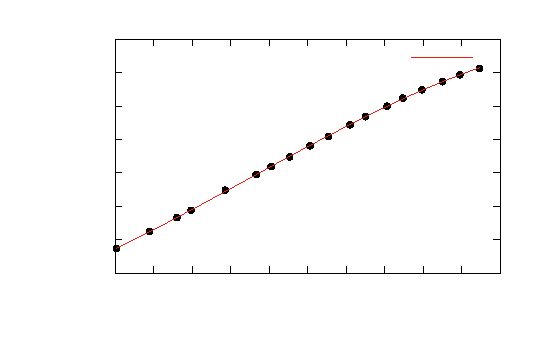
\includegraphics[width={252.00bp},height={158.40bp}]{pole}}%
    \gplfronttext
  \end{picture}%
\endgroup
 }
        \captionsetup{type=graph}
        \caption{Graf závislosti intenzity magnetického pole na proudu. }
    \end{minipage} 
\end{table}

\subsection{Ověření funkčnosti Fabry-Perotova interferometru}

Elektromagnety jsem zatím nechal vypnuté a vyfotil interferenční obrazec nerozštěpené spektrální čáry. Ze vztahu (1) vyplývá, že pokud pozorujeme paprsky pohybující se pod malými úhly $ \Theta_m $, bude $ m \approx \frac{2nd}{\lambda} $, takže nějaké velké  číslo, které není jednoduché zjistit. Zárověň podle vztahu (1) by měly poloměry kroužků s rostoucím $ m $ klesat, takže ty kroužky které vidím přeindexuju od nejmenšího s $ m_0 = m_{max} $  jako $ m = m_{max} - p $.  
Aby naměřená data odpovídala vztahu (3), musí být závislost lineární, což se podařilo ověřit a můžu přejít k měření štěpení spektrálních čar. 

\begin{equation}
    a = \frac{(fZ)^2n \lambda}{d} = (86 \pm 1) \cdot 10^{-9} \text{ m}^2
\end{equation}

\begin{figure}[htpb]
    \centering
    % GNUPLOT: LaTeX picture with Postscript
\begingroup
  \makeatletter
  \providecommand\color[2][]{%
    \GenericError{(gnuplot) \space\space\space\@spaces}{%
      Package color not loaded in conjunction with
      terminal option `colourtext'%
    }{See the gnuplot documentation for explanation.%
    }{Either use 'blacktext' in gnuplot or load the package
      color.sty in LaTeX.}%
    \renewcommand\color[2][]{}%
  }%
  \providecommand\includegraphics[2][]{%
    \GenericError{(gnuplot) \space\space\space\@spaces}{%
      Package graphicx or graphics not loaded%
    }{See the gnuplot documentation for explanation.%
    }{The gnuplot epslatex terminal needs graphicx.sty or graphics.sty.}%
    \renewcommand\includegraphics[2][]{}%
  }%
  \providecommand\rotatebox[2]{#2}%
  \@ifundefined{ifGPcolor}{%
    \newif\ifGPcolor
    \GPcolorfalse
  }{}%
  \@ifundefined{ifGPblacktext}{%
    \newif\ifGPblacktext
    \GPblacktexttrue
  }{}%
  % define a \g@addto@macro without @ in the name:
  \let\gplgaddtomacro\g@addto@macro
  % define empty templates for all commands taking text:
  \gdef\gplbacktext{}%
  \gdef\gplfronttext{}%
  \makeatother
  \ifGPblacktext
    % no textcolor at all
    \def\colorrgb#1{}%
    \def\colorgray#1{}%
  \else
    % gray or color?
    \ifGPcolor
      \def\colorrgb#1{\color[rgb]{#1}}%
      \def\colorgray#1{\color[gray]{#1}}%
      \expandafter\def\csname LTw\endcsname{\color{white}}%
      \expandafter\def\csname LTb\endcsname{\color{black}}%
      \expandafter\def\csname LTa\endcsname{\color{black}}%
      \expandafter\def\csname LT0\endcsname{\color[rgb]{1,0,0}}%
      \expandafter\def\csname LT1\endcsname{\color[rgb]{0,1,0}}%
      \expandafter\def\csname LT2\endcsname{\color[rgb]{0,0,1}}%
      \expandafter\def\csname LT3\endcsname{\color[rgb]{1,0,1}}%
      \expandafter\def\csname LT4\endcsname{\color[rgb]{0,1,1}}%
      \expandafter\def\csname LT5\endcsname{\color[rgb]{1,1,0}}%
      \expandafter\def\csname LT6\endcsname{\color[rgb]{0,0,0}}%
      \expandafter\def\csname LT7\endcsname{\color[rgb]{1,0.3,0}}%
      \expandafter\def\csname LT8\endcsname{\color[rgb]{0.5,0.5,0.5}}%
    \else
      % gray
      \def\colorrgb#1{\color{black}}%
      \def\colorgray#1{\color[gray]{#1}}%
      \expandafter\def\csname LTw\endcsname{\color{white}}%
      \expandafter\def\csname LTb\endcsname{\color{black}}%
      \expandafter\def\csname LTa\endcsname{\color{black}}%
      \expandafter\def\csname LT0\endcsname{\color{black}}%
      \expandafter\def\csname LT1\endcsname{\color{black}}%
      \expandafter\def\csname LT2\endcsname{\color{black}}%
      \expandafter\def\csname LT3\endcsname{\color{black}}%
      \expandafter\def\csname LT4\endcsname{\color{black}}%
      \expandafter\def\csname LT5\endcsname{\color{black}}%
      \expandafter\def\csname LT6\endcsname{\color{black}}%
      \expandafter\def\csname LT7\endcsname{\color{black}}%
      \expandafter\def\csname LT8\endcsname{\color{black}}%
    \fi
  \fi
    \setlength{\unitlength}{0.0500bp}%
    \ifx\gptboxheight\undefined%
      \newlength{\gptboxheight}%
      \newlength{\gptboxwidth}%
      \newsavebox{\gptboxtext}%
    \fi%
    \setlength{\fboxrule}{0.5pt}%
    \setlength{\fboxsep}{1pt}%
    \definecolor{tbcol}{rgb}{1,1,1}%
\begin{picture}(5040.00,3168.00)%
    \gplgaddtomacro\gplbacktext{%
      \csname LTb\endcsname%%
      \put(946,704){\makebox(0,0)[r]{\strut{}$0$}}%
      \put(946,984){\makebox(0,0)[r]{\strut{}$0.05$}}%
      \put(946,1265){\makebox(0,0)[r]{\strut{}$0.1$}}%
      \put(946,1545){\makebox(0,0)[r]{\strut{}$0.15$}}%
      \put(946,1826){\makebox(0,0)[r]{\strut{}$0.2$}}%
      \put(946,2106){\makebox(0,0)[r]{\strut{}$0.25$}}%
      \put(946,2386){\makebox(0,0)[r]{\strut{}$0.3$}}%
      \put(946,2667){\makebox(0,0)[r]{\strut{}$0.35$}}%
      \put(946,2947){\makebox(0,0)[r]{\strut{}$0.4$}}%
      \put(1078,484){\makebox(0,0){\strut{}$1$}}%
      \put(1969,484){\makebox(0,0){\strut{}$2$}}%
      \put(2861,484){\makebox(0,0){\strut{}$3$}}%
      \put(3752,484){\makebox(0,0){\strut{}$4$}}%
      \put(4643,484){\makebox(0,0){\strut{}$5$}}%
    }%
    \gplgaddtomacro\gplfronttext{%
      \csname LTb\endcsname%%
      \put(209,1825){\rotatebox{-270}{\makebox(0,0){\strut{}$ r_p^2 $ (mm$ ^2$)}}}%
      \put(2860,154){\makebox(0,0){\strut{}p}}%
      \csname LTb\endcsname%%
      \put(3656,2774){\makebox(0,0)[r]{\strut{}fit $ ax + b $}}%
    }%
    \gplbacktext
    \put(0,0){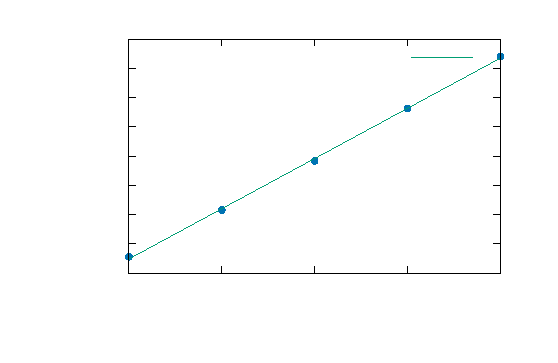
\includegraphics[width={252.00bp},height={158.40bp}]{fabry}}%
    \gplfronttext
  \end{picture}%
\endgroup

    \captionsetup{type=graph}
    \caption{Závislost čtverce poloměru kroužků na indexu p}
\end{figure}

\subsection{Bohrův magneton}

Tentokrát jsem cívkami nechal téct proud $ I $ a pomalu ho zvyšoval, než se kolem $ I = 5 A $ začaly interferenční kroužky viditelně dělit na tři. Pro několik hodnot proudu jsem potom měřil poloměry vsěch kroužků o třech různých řádech, takže celkem 9 poloměrů číslovaných od $ R_1 $ do $ R_9 $. Výsledný rozdíl energií od střední $ \pi $ čáry je potom dopočítaný podle vztahu (5) a všechna data jsou uvedená v Tabulce 2. 

\begin{table}[h]
    \centering
    \small
    \begin{tabular}{ | c | c c c | c c | }
        \hline
        $ I $ (A) & $ R_3 $ (mm) & $ R_2 $ (mm) & $ R_1 $ (mm) & $ \Delta E_1 \cdot 10^{-24} $ (J) &  $ \Delta E_2 \cdot 10t^{-24} $ (J)  \\
        \hline
        4.94 & 0.1963 & 0.1652 & 0.1248 & 2.982 & 3.108 \\
        5.85 & 0.2013 & 0.1630 & 0.1201 & 3.702 & 3.222 \\
        6.58 & 0.2060 & 0.1820 & 0.1144 & 2.470 & 5.316 \\
        7.45 & 0.2098 & 0.1630 & 0.1065 & 4.629 & 4.040 \\
        8.36 & 0.2145 & 0.1653 & 0.0997 & 4.957 & 4.612 \\
        9.38 & 0.2169 & 0.1646 & 0.0897 & 5.293 & 5.053 \\
        \hline                                 
        $ I $ (A) & $ R_6 $ (mm) & $ R_5              $ (mm) & $ R_4 $  (mm) & $ \Delta E_1 \cdot 10^{-24} $ (J) &  $ \Delta E_2 \cdot 10t^{-24} $ (J)    \\
        \hline                          
        4.94 & 0.3454 & 0.3267 & 0.3081 & 3.334 & 3.132 \\
        5.85 & 0.3469 & 0.3298 & 0.3055 & 3.070 & 4.096 \\
        6.58 & 0.3491 & 0.3295 & 0.3026 & 3.529 & 4.511 \\
        7.45 & 0.3542 & 0.3284 & 0.3008 & 4.672 & 4.607 \\
        8.36 & 0.3567 & 0.3273 & 0.2990 & 5.335 & 4.702 \\
        9.38 & 0.3572 & 0.3284 & 0.2966 & 5.238 & 5.273 \\
        \hline                                 
        $ I $ (A) & $ R_9 $ (mm) & $ R_8              $ (mm) & $ R_7 $  (mm) & $ \Delta E_1 \cdot 10^{-24} $ (J) &  $ \Delta E_2 \cdot 10t^{-24} $ (J)   \\
        \hline                          
        4.94 & 0.4530 & 0.4376 & 0.4238 & 3.639 & 3.154 \\ 
        5.85 & 0.4537 & 0.4379 & 0.4224 & 3.737 & 3.538 \\ 
        6.58 & 0.4564 & 0.4393 & 0.4159 & 4.063 & 5.309 \\ 
        7.45 & 0.4574 & 0.4374 & 0.4158 & 4.748 & 4.889 \\ 
        8.36 & 0.4599 & 0.4384 & 0.4152 & 5.124 & 5.254 \\ 
        9.38 & 0.4634 & 0.4384 & 0.4121 & 5.981 & 5.934 \\ 
        \hline
    \end{tabular}
    \caption{Naměřená data Zeemanova jevu}
\end{table}

Získané rozdíly energie jsou vykreslené do Grafu 3 v závislosti na intenzitě magnetické indukce $ B $ a výsledná závislost je fitovaná přímkou podle vztahu (10), odkud vychází výsledná hodnota Bohrova magentonu

\begin{equation}
\mu_B = (10.2 \pm 0.7) 10^{-24} \text{ Am}^2
\end{equation}

\begin{figure}[htpb]
    \centering
    % GNUPLOT: LaTeX picture with Postscript
\begingroup
  \makeatletter
  \providecommand\color[2][]{%
    \GenericError{(gnuplot) \space\space\space\@spaces}{%
      Package color not loaded in conjunction with
      terminal option `colourtext'%
    }{See the gnuplot documentation for explanation.%
    }{Either use 'blacktext' in gnuplot or load the package
      color.sty in LaTeX.}%
    \renewcommand\color[2][]{}%
  }%
  \providecommand\includegraphics[2][]{%
    \GenericError{(gnuplot) \space\space\space\@spaces}{%
      Package graphicx or graphics not loaded%
    }{See the gnuplot documentation for explanation.%
    }{The gnuplot epslatex terminal needs graphicx.sty or graphics.sty.}%
    \renewcommand\includegraphics[2][]{}%
  }%
  \providecommand\rotatebox[2]{#2}%
  \@ifundefined{ifGPcolor}{%
    \newif\ifGPcolor
    \GPcolorfalse
  }{}%
  \@ifundefined{ifGPblacktext}{%
    \newif\ifGPblacktext
    \GPblacktexttrue
  }{}%
  % define a \g@addto@macro without @ in the name:
  \let\gplgaddtomacro\g@addto@macro
  % define empty templates for all commands taking text:
  \gdef\gplbacktext{}%
  \gdef\gplfronttext{}%
  \makeatother
  \ifGPblacktext
    % no textcolor at all
    \def\colorrgb#1{}%
    \def\colorgray#1{}%
  \else
    % gray or color?
    \ifGPcolor
      \def\colorrgb#1{\color[rgb]{#1}}%
      \def\colorgray#1{\color[gray]{#1}}%
      \expandafter\def\csname LTw\endcsname{\color{white}}%
      \expandafter\def\csname LTb\endcsname{\color{black}}%
      \expandafter\def\csname LTa\endcsname{\color{black}}%
      \expandafter\def\csname LT0\endcsname{\color[rgb]{1,0,0}}%
      \expandafter\def\csname LT1\endcsname{\color[rgb]{0,1,0}}%
      \expandafter\def\csname LT2\endcsname{\color[rgb]{0,0,1}}%
      \expandafter\def\csname LT3\endcsname{\color[rgb]{1,0,1}}%
      \expandafter\def\csname LT4\endcsname{\color[rgb]{0,1,1}}%
      \expandafter\def\csname LT5\endcsname{\color[rgb]{1,1,0}}%
      \expandafter\def\csname LT6\endcsname{\color[rgb]{0,0,0}}%
      \expandafter\def\csname LT7\endcsname{\color[rgb]{1,0.3,0}}%
      \expandafter\def\csname LT8\endcsname{\color[rgb]{0.5,0.5,0.5}}%
    \else
      % gray
      \def\colorrgb#1{\color{black}}%
      \def\colorgray#1{\color[gray]{#1}}%
      \expandafter\def\csname LTw\endcsname{\color{white}}%
      \expandafter\def\csname LTb\endcsname{\color{black}}%
      \expandafter\def\csname LTa\endcsname{\color{black}}%
      \expandafter\def\csname LT0\endcsname{\color{black}}%
      \expandafter\def\csname LT1\endcsname{\color{black}}%
      \expandafter\def\csname LT2\endcsname{\color{black}}%
      \expandafter\def\csname LT3\endcsname{\color{black}}%
      \expandafter\def\csname LT4\endcsname{\color{black}}%
      \expandafter\def\csname LT5\endcsname{\color{black}}%
      \expandafter\def\csname LT6\endcsname{\color{black}}%
      \expandafter\def\csname LT7\endcsname{\color{black}}%
      \expandafter\def\csname LT8\endcsname{\color{black}}%
    \fi
  \fi
    \setlength{\unitlength}{0.0500bp}%
    \ifx\gptboxheight\undefined%
      \newlength{\gptboxheight}%
      \newlength{\gptboxwidth}%
      \newsavebox{\gptboxtext}%
    \fi%
    \setlength{\fboxrule}{0.5pt}%
    \setlength{\fboxsep}{1pt}%
    \definecolor{tbcol}{rgb}{1,1,1}%
\begin{picture}(5328.00,3600.00)%
    \gplgaddtomacro\gplbacktext{%
      \csname LTb\endcsname%%
      \put(814,704){\makebox(0,0)[r]{\strut{}$2$}}%
      \put(814,1038){\makebox(0,0)[r]{\strut{}$2.5$}}%
      \put(814,1373){\makebox(0,0)[r]{\strut{}$3$}}%
      \put(814,1707){\makebox(0,0)[r]{\strut{}$3.5$}}%
      \put(814,2042){\makebox(0,0)[r]{\strut{}$4$}}%
      \put(814,2376){\makebox(0,0)[r]{\strut{}$4.5$}}%
      \put(814,2710){\makebox(0,0)[r]{\strut{}$5$}}%
      \put(814,3045){\makebox(0,0)[r]{\strut{}$5.5$}}%
      \put(814,3379){\makebox(0,0)[r]{\strut{}$6$}}%
      \put(946,484){\makebox(0,0){\strut{}$250$}}%
      \put(1743,484){\makebox(0,0){\strut{}$300$}}%
      \put(2540,484){\makebox(0,0){\strut{}$350$}}%
      \put(3337,484){\makebox(0,0){\strut{}$400$}}%
      \put(4134,484){\makebox(0,0){\strut{}$450$}}%
      \put(4931,484){\makebox(0,0){\strut{}$500$}}%
    }%
    \gplgaddtomacro\gplfronttext{%
      \csname LTb\endcsname%%
      \put(209,2041){\rotatebox{-270}{\makebox(0,0){\strut{}$ | \Delta E | $ (J) }}}%
      \put(2938,154){\makebox(0,0){\strut{}$ B $ (mT)}}%
      \csname LTb\endcsname%%
      \put(3944,3206){\makebox(0,0)[r]{\strut{}fit}}%
    }%
    \gplbacktext
    \put(0,0){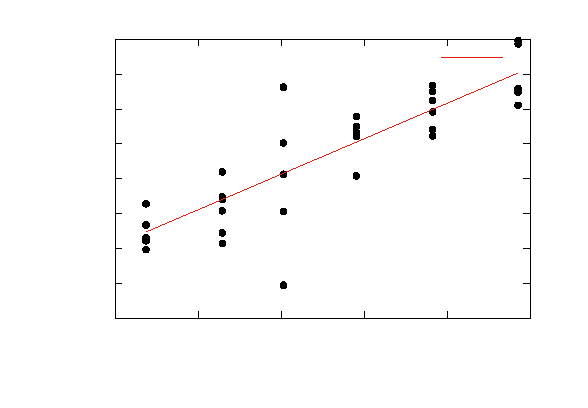
\includegraphics[width={266.40bp},height={180.00bp}]{magneton}}%
    \gplfronttext
  \end{picture}%
\endgroup

    \captionsetup{type=graph}
    \caption{ Graf závislosti rozdílu energie fotonů oproti základnímu přechodu na intenzitě magnetického pole v lampě.   }
\end{figure}

\subsection{Polarizace spektrálních čar}

Když pozorujeme kadmiovou lampu ve směru kolmém na magentickou indukci, měly by podle teorie být paprsky odpovídající $ \pi $ i $ \sigma $ polarizované lineárně. $ \pi $ rovnoběžně s $ \vec{B} $ a $ \sigma $ kolmo. Pro ověření této skutečnosti stačí vzít polarizační filtr a umístit ho před kameru. Pokud byla osa polarizátoru souběžná s $ \vec{B} $, byla vidět jen střední čára, pokud byla kolmá byly vidět jen dvě vnější. 

V případě pozorování světla ze směru rovnoběžného s magnetickou indukcí by střední čára neměla být vidět vůbec a ostatní dvě by měly mít kruhovou polarizaci s opačnou točivostí. Když jsem otočil stolek s lampou o $ 90 ^{\circ} $, tak opravdu prostřední čára zmizela a vnější dvě čáry měly stejnou intenzitu bez ohledu na otočení polarizátoru. K ověření, že jde o kruhovou polarizaci je možné použít čtvrtvlnnou destičku, která kruhově polarizované světlo převede na lineárně polarizované a o tom se dá zase rozhodnout polarizačním filterm. Při jeho otáčení uvidíme dvě maxima od sebe otočené o $ 90 ^{\circ} $ což odpovídá různé točivosti polarizací. 

\subsection{Anomální Zeemanův jev}

Ve spektru kadmia se nachází i spektrální čára o vlnové délce $ \lambda = 508.588 $ nm, která vzniká při přechodu $ 4d^{10}5s6s \to  4d^{10}5s5p $. V tomto případě je celkový spinový moment nenulový a proto se v magnetickém poli tato čára štěpí anomálně. Na optickou lavici jsem umístil zelený filtr místo červeného a při zapnutí magnetického pole by se mělo vzniknout 9 různých spektrálních čar. Ty ale nebyli příliš dobře rozlišitelné. 


\section{Závěr}

V tomto praktiku jsem pomocí Fabry-Perotova interferometru ověřil, že štěpení energiových hladin spektrálních čar při normálním Zeemanově jevu se řídí lineárním vztahem (10) a zněj byl určený Bohrův magneton $ \mu_B = (10.2 \pm 0.7) 10^{-24} $ Am$ ^2 $, zatímco tabulková hodnota je $ \mu_B = 9.274 \cdot 10^{-24} $ Am$ ^2 $. Největším důvodem chyby je pravděpodobně nepřesné odečítání poloměrů kružnic v interferenčním obrazci, protože ne vždycky byli přesné kružnice a nebyli příliš ostré.


V druhé části úlohy jsem ověřil, že polarizace pozorovaných spektrálních čar odpovídá teorii.

\begin{thebibliography}{0}
\bibitem{tabulky} Návod k úloze~\url{https://is.muni.cz/auth/el/sci/jaro2025/F4210/um/fp3-6_Zeeman.pdf}.   
\end{thebibliography}

\end{document}
